\chapter{Implementacja}

\section{Architektura}

\section{Web serwisy}
\subsection{Web serwis przyjmujący zadania}

\subsection{Web serwis przyjmujący wyniki}

\section{Format danych}

\subsection{GEXF}

\section{Algorytmy}

\subsection{BFS}

\subsection{DFS}

\subsection{A*}

\subsection{Bellman-Ford}

\subsection{Dijkstra}

\subsection{Uniform Cost}

\subsection{Floyd-Warshall}

\subsection{Prim}
aa

\subsection{Kruskal}

\section{Metryki}

\subsection{Czas wykonania}

\subsection{Zużycie pamięci}

\subsection{Waga ścieżki}

\section{Enterprise Integration Patterns}
W naszym projekcie wykorzystaliśmy cztery różne biblioteki do obliczeń grafowych. 
Każda z nich posiadała inną reprezentację danych. Wykorzystane biblioteki to:

\begin{itemize}
 \item JUNG
 \item GeoTools
 \item aima-java
 \item JGraphT
\end{itemize}

Aby umożliwić wykorzystanie algorytmów pochodzących z tych bibliotek, potrzebne było dokonanie transformacji przychodzących danych wejściowych z
formatu GEXF do formatu wykorzystywanego przez daną bibliotekę.
W tym celu skorzystaliśmy ze wzorców projektowych Enterprise Integration Patterns zaproponowanych w \cite{hohpe2004enterprise}.

\subsection{Normalizer}
Wzorzec projektowy Normalizer wykorzystuje Message Router aby skierować przychodzącą wiadomość do odpowiadającego jej Message Translatora.
Wymaga to, aby Message Router wykrył typ przesłanej wiadomości i na tej podstawie skierował ją w odopowienie miejsce.
Sytuacja została przedstawiona na rysunku \ref{fig:normalizer}

\begin{figure}[!h]
 \centering
 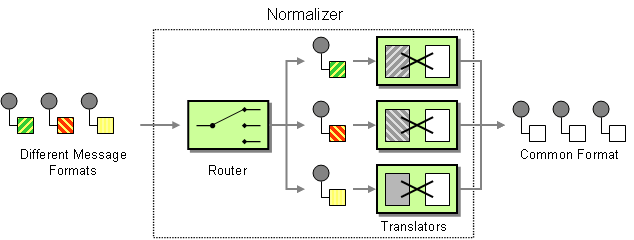
\includegraphics[width=1.0\textwidth]{eip/Normalizer}
 \caption{Wzorzec Normalizer}
 \label{fig:normalizer}
\end{figure}

\subsection{Message Router}
Worzec Message Router zapewnia przekazanie przychodzącej wiadomości do odpowiedniej kolejki w której odbędzie się dalsze przetwarzanie wiadomości.
Dokonuje się to, na podstawie wykrytego typu wiadomości.
Sytuacja została przedstawiona na rysunku \ref{fig:messageRouter}

\begin{figure}[!h]
 \centering
 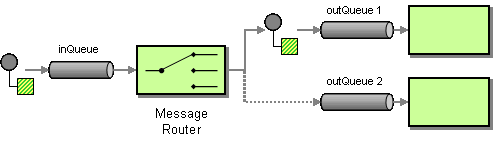
\includegraphics[width=1.0\textwidth]{eip/MessageRouter}
 \caption{Wzorzec Message Router}
 \label{fig:messageRouter}
\end{figure}

\subsection{Message Translator}
Wzorzec projektowy Message Translator wykorzystywany jest do transformacji przychodzącej wiadomości do określonego formatu wyjściowego.
Symbolicznie zostało to przedstawione na rysunku \ref{fig:messageTranslator}

\begin{figure}[!h]
 \centering
 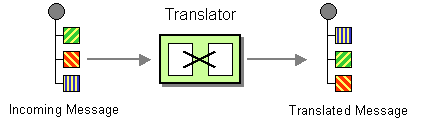
\includegraphics[width=1.0\textwidth]{eip/MessageTranslator}
 \caption{Wzorzec Message Translator}
 \label{fig:messageTranslator}
\end{figure}

\section{Uruchamianie zadań}
